
\begin{document}

\begin{frame}{Структура органов власти}

\insertpicc{emil/vlast.jpg}
    
\end{frame}

\begin{frame}{Дом республики}

\insertpicc{emil/adminka.jpg}
    
\end{frame}

\begin{frame}{Первый президент республики Башкортостан}

\begin{figure}[h!]
	\begin{center}
		{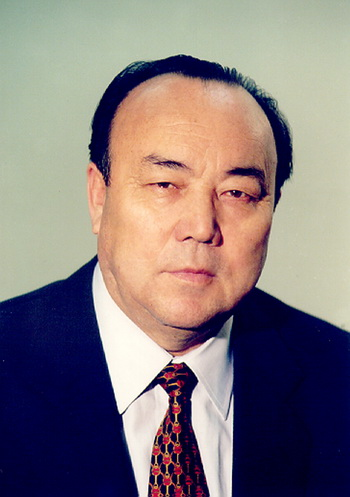
\includegraphics[width=0.5\linewidth]{emil/M_G_Rakhimov.jpg}}
		\caption{Районы Башкоростана}
	\end{center}
\end{figure}

\end{frame}


\begin{frame}{Первый президент республики Башкортостан}

\begin{figure}[h!]
	\begin{center}
		{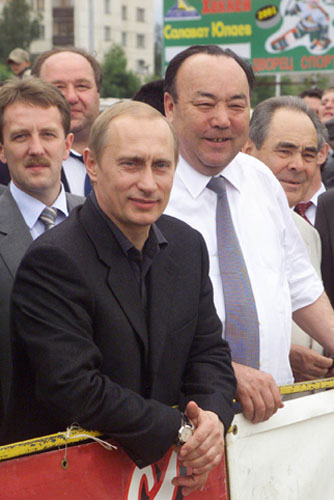
\includegraphics[width=0.4\linewidth]{emil/Murtaza_Rakhimov_and_Vladimir_Putin.jpg}}
		\caption{Муртаза Губайдулович Рахимов и Владимир Владимирович Путин}
	\end{center}
\end{figure}

\end{frame}

\begin{frame}{Заслуги}

\begin{itemize}
	\item Построено более 1000 школ
	\item В школах дети 15 национальностей имеют возможность изучать родной язык
	\item Республика входила в список регионов-доноров до 2006 года. И вновь вошла в список доноров в 2011 году, и входит в этот список до сих пор
	\item На июнь 2009 республика не входила в список кризисных
	\item За оказанную поддержку православной религии в республике Башкортостан, имя Муртазы Рахимова отлито на одном из колоколов собора Рождества Богородицы в Уфе
\end{itemize}

\end{frame}

\begin{frame}{Критика центральных властей}

\begin{itemize}
	\item Муртаза Рахимов о партии «Единая Россия»: «Партией пытаются рулить люди, которые и тремя курицами не командовали»
	\item Муртаза Рахимов: «С регионами легко стали делиться социальными обязательствами перед людьми, но не доходами»
\end{itemize}

\end{frame}

\begin{frame}{Что имеем на самом деле}

В России лишь чуть более десятка субъектов федерации обладает собственным крупным нефтяным потенциалом – только в 12 регионах добывается 10 и более миллионов тонн нефти в год.

\begin{itemize}
	\item среднедушевые доходы в последние 20 лет всегда были и есть ниже среднероссийских: по этому показателю республика занимает 22-е место в стране
	\item  по среднемесячному размеру назначенных пенсий республика на 60-м (!) месте среди субъектов Российской Федерации.
	\item по социальному расслоению Башкирия на седьмом месте в России, коэффициент дифференциации доходов 18,5, против 16,9 в среднем по России
\end{itemize}

\end{frame}

\begin{frame}{Что имеем}

\begin{figure}[h!]
	\begin{center}
		{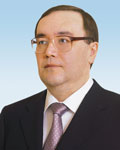
\includegraphics[width=0.25\linewidth]{emil/RahimovUM.jpg}}
		\caption{Рахимов Урал, В 2005—2012 годы входил в список 200 богатейших бизнесменов России по версии журнала Forbes}
	\end{center}
\end{figure}

После смены собственника «Башнефти» наблюдается взрывной рост платежей по налогу на прибыль: по данным компании за первый квартал 2010 года, они выросли в сравнении с I кварталом 2009 года в 12 (!) раз, что позволяет оценить масштаб занижения налога на прибыль в предыдущие годы. 
\end{frame}

\begin{frame}{Второй президент республики Башкортостан}

\begin{figure}[h!]
	\begin{center}
		{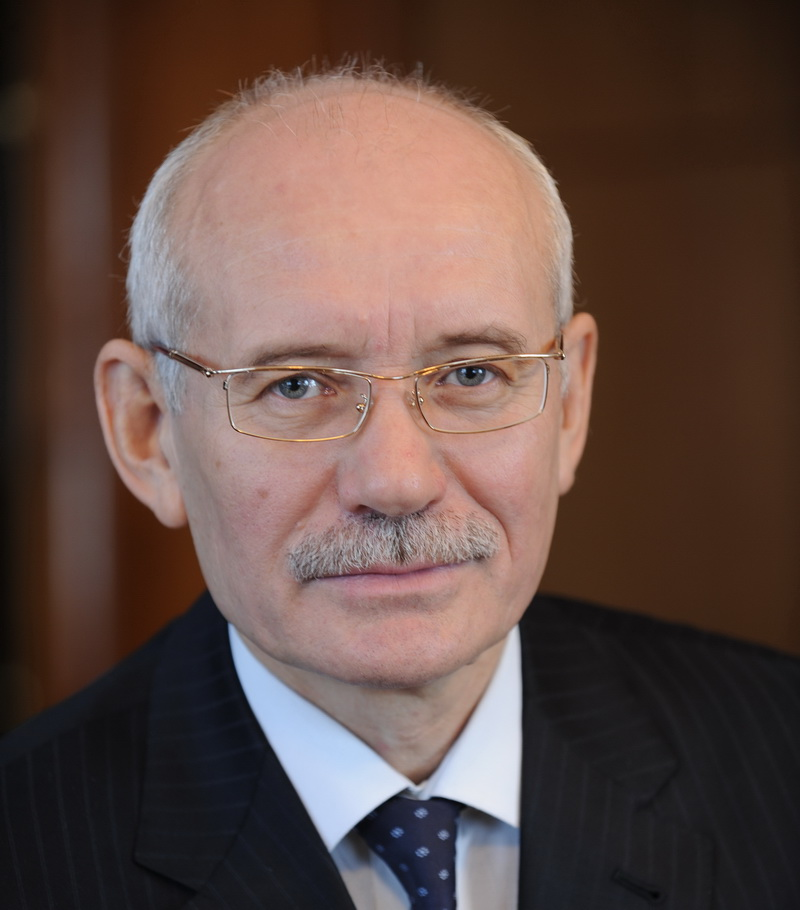
\includegraphics[width=0.5\linewidth]{emil/Rustem_Khamitov.jpg}}
		\caption{Хамитов Рустэм Закиевич}
	\end{center}
\end{figure}

\end{frame}

\begin{frame}{Положительные моменты правления}

\begin{itemize}
	\item  ВРП региона вырос с 759,2 млрд рублей в 2010 году до 1 трлн 343,9 млрд в 2014
	\item уменьшилась доля добычи полезных ископаемых в структуре валового продукта региона, если в 2009 году она составляла 8,1 \%67, то в 2012 году уже 2,9 \%68
	\item спустя 10 месяцев после вступления Рустэма Хамитова в должность Президента Башкортостана, международное рейтинговое агентство Standard & Poor’s (S&P) повысило долгосрочный кредитный рейтинг республики со «стабильного» (BB-) на «позитивный» (BB+)
	\item в 2012 году Башкортостан получил высшую оценку Национального рейтинга прозрачности закупок — «Гарантированная прозрачность», переместившись с 34-го места по этому показателю на второе
\end{itemize}

\end{frame}

\begin{frame}{Отрицательные моменты правления}

\begin{itemize}
	\item  в 2010 году долг составлял 6,9 млрд рублей (1 \% от ВРП), то к концу 2013 года он дошёл до 19,8 млрд рублей
	\item увеличение дефицита бюджета региона: в 2010 году — 3,4 млрд рублей; в 2014 — 15 млрд рублей
	\item  в период нахождения Хамитова на посту главы региона наблюдается отрицательный прирост населения, что может являться показателем неблагоприятной экономической ситуации
	\item регион из энергодостаточного превратился в энергодефицитный. Если в 2011 году потребление электроэнергии на 2,4 \% опережало производство, то в 2015 году наметился дефицит в 16,5 \%
	\item обострениt проблем с коррупцией, особенно в сфере ЖКХ
\end{itemize}

\end{frame}

\end{document}